\section{Model}
\label{sec:model}

% A general model family - conditional exponential models
% Incorporating feedback as "measurements" as per Percy
% Error model - defer investigation to a later section.
% Querying for an optimal measurement - defer asynchrony to a later section.
% Learning given feedback 

Our goal, given an existing model, is to identify labels where we lack confidence, query crowd works for measurements if needed and incorporate the resultant responses back into our model.
We consider the family of conditional exponential models, a popular class of models that include logistic regression and conditional random fields.
Let $\bx$ be given input, then the labels $\by = y_1, \ldots, y_n$ is generated by the following conditional distribution:
\begin{align*}
  \p(\by \given \bx) 
  &= \exp( \theta^\top \phi(\bx, \by) - A(\theta; \bx)),
\end{align*}
where $\theta$ are the model parameters, $\phi(\bx, \by)$ are arbitrary features of the input and labels and $A(\theta; x)$ is the conditional log-normalizer.
We assume that the model has low treewidth (e.g.\ $\phi$ factorizes over the labels $\by$) or otherwise admits efficient marginal computation.
In our running example of information extraction from classifieds, the model is a linear-chain conditional random field (\figureref{crf}).

\begin{figure}[t]
  \begin{centering}
  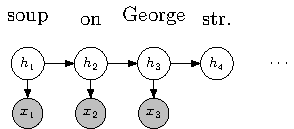
\includegraphics[width=0.5\textwidth]{figures/simple-crf.pdf}
  \end{centering}
  \caption{A conditional random field \todo{(arun): make a CRF and show what happens when measurements are added.}}
  \label{fig:crf}
\end{figure}

Conventionally, we are given a training dataset $\sD = \{\bx_i, \by_i\}$ and can learn $\theta$ by optimizing the convex log-likelihood objective $\sL(\theta) = \sum_{t=1}^T \log \p(\by\oft{t} \given \bx\oft{t})$.
In our setting, however, we do not observe the gold labels $\by$. 
Instead, we can ask the crowd to provide a ``measurement'' for some subset of the labels.
Let $\Sigma = \{\sigma_i\}$ be the set of possible measurements we can ask the crowd for and 
let $\by_\sigma \subseteq \by$ be the subset of labels queried.
The responses, $\tau_\sigma$, are modeled with an exponential measurement model as in~\cite{liang09measurements}:
\begin{align*}
  p(\tau_\sigma \given x, y) 
  &\propto \exp \left( \theta'^\top\phi'(\tau_\sigma, \bx, \by_\sigma) \right),
\end{align*}
where $\theta'$ and $\phi'$ are extra parameters and features.
The choice of an exponential model allows us to simply include measurements as an additional factor.
\figureref{crf} shows the original graph with additional measurement nodes.

\todo{arun: maybe this goes to the human errors section}
In the simplest case, assume the labeler returns the true label with a uniform probability of $1- \epsilon$, and guesses at random otherwise, $\theta'$ and $\phi'$ are:
\begin{align*}
  \theta' &= 
      \begin{bmatrix}
        1 - \e \\ \e
      \end{bmatrix} &
  \phi'(\tau_\sigma, \by_\sigma, \bx) &=
    \begin{bmatrix}
      \BI[\tau_\sigma = y_\sigma] \\
      \BI[\tau_\sigma \neq y_\sigma]
    \end{bmatrix}.
\end{align*}
Independently, we model the time each measurement takes, $D_\sigma$.
We revisit the problem of learning the error distribution of labelers in \sectionref{human-error}.

Next, we describe how we use our models to predict labels and learn from partial feedback.

\paragraph{Prediction}
Given parameters $\theta$ and measurement responses  $\tau_1, \ldots, \tau_n$, we query for predictions using a maximum likelihood labeling:
$\byt \given \bx, \tau_1, \ldots \tau_n = \argmax_{\by} \p(\by \given \bx, \tau_1, \ldots \tau_n)$.

\paragraph{Learning from responses}

Recall that we do not have gold labels for our data, but only noisy measurements: we do not have supervised examples to do training from. 
Under the assumption that the measurements from people are highly correlated with the gold labels, we use (online) expectation-maximization to jointly learn parameters for our model and the human error model.
